% THIS IS SIGPROC-SP.TEX - VERSION 3.1
% WORKS WITH V3.2SP OF ACM_PROC_ARTICLE-SP.CLS
% APRIL 2009
%
% It is an example file showing how to use the 'acm_proc_article-sp.cls' V3.2SP
% LaTeX2e document class file for Conference Proceedings submissions.
% ----------------------------------------------------------------------------------------------------------------
% This .tex file (and associated .cls V3.2SP) *DOES NOT* produce:
%       1) The Permission Statement
%       2) The Conference (location) Info information
%       3) The Copyright Line with ACM data
%       4) Page numbering
% ---------------------------------------------------------------------------------------------------------------
% It is an example which *does* use the .bib file (from which the .bbl file
% is produced).
% REMEMBER HOWEVER: After having produced the .bbl file,
% and prior to final submission,
% you need to 'insert'  your .bbl file into your source .tex file so as to provide
% ONE 'self-contained' source file.
%
% Questions regarding SIGS should be sent to
% Adrienne Griscti ---> griscti@acm.org
%
% Questions/suggestions regarding the guidelines, .tex and .cls files, etc. to
% Gerald Murray ---> murray@hq.acm.org
%
% For tracking purposes - this is V3.1SP - APRIL 2009

\documentclass{acm_proc_article-sp}

\begin{document}

\title{Pollination in MAIDS: Detecting and Combating\\Passive Intrusions in a Multi-Agent System}
% \subtitle{[Extended Abstract]
% \titlenote{A full version of this paper is available as
% \textit{Author's Guide to Preparing ACM SIG Proceedings Using
% \LaTeX$2_\epsilon$\ and BibTeX} at
% \texttt{www.acm.org/eaddress.htm}}}
%
% You need the command \numberofauthors to handle the 'placement
% and alignment' of the authors beneath the title.
%
% For aesthetic reasons, we recommend 'three authors at a time'
% i.e. three 'name/affiliation blocks' be placed beneath the title.
%
% NOTE: You are NOT restricted in how many 'rows' of
% "name/affiliations" may appear. We just ask that you restrict
% the number of 'columns' to three.
%
% Because of the available 'opening page real-estate'
% we ask you to refrain from putting more than six authors
% (two rows with three columns) beneath the article title.
% More than six makes the first-page appear very cluttered indeed.
%
% Use the \alignauthor commands to handle the names
% and affiliations for an 'aesthetic maximum' of six authors.
% Add names, affiliations, addresses for
% the seventh etc. author(s) as the argument for the
% \additionalauthors command.
% These 'additional authors' will be output/set for you
% without further effort on your part as the last section in
% the body of your article BEFORE References or any Appendices.

\numberofauthors{4} %  in this sample file, there are a *total*
% of EIGHT authors. SIX appear on the 'first-page' (for formatting
% reasons) and the remaining two appear in the \additionalauthors section.
%
\author{
% You can go ahead and credit any number of authors here,
% e.g. one 'row of three' or two rows (consisting of one row of three
% and a second row of one, two or three).
%
% The command \alignauthor (no curly braces needed) should
% precede each author name, affiliation/snail-mail address and
% e-mail address. Additionally, tag each line of
% affiliation/address with \affaddr, and tag the
% e-mail address with \email.
%
% 1st. author
\alignauthor
Jeremy Kackley\\
       \affaddr{Noetic Strategies, Inc}\\
       \affaddr{P.O. Box 22225}\\
       \affaddr{Huntsville, AL 35814}\\
       \email{jeremy.kackley@gmail.com}
% 2nd. author
\alignauthor
James Jacobs\\
       \affaddr{Jackson State University/CDID}\\
       \affaddr{1230 Raymond Rd.}\\
       \affaddr{Jackson, MS 39204}\\
       \email{jjacobs@c-did.com}
% 3rd. author
\alignauthor 
Paulus Wahjudi\\
       \affaddr{Weisberg Division of Engineering \& Computer Science}\\
       \affaddr{Marshall University}\\
       \affaddr{Huntington, WV 25755}\\
       \email{wahjudi@marshall.edu}
% \and  % use '\and' if you need 'another row' of author names
% 4th. author
\and
\alignauthor 
Jean Gourd\\
       \affaddr{Louisiana Tech University}\\
       \affaddr{Center for Secure Cyberspace}\\
       \affaddr{P.O. Box 10348}\\
       \affaddr{Ruston, LA 71272}\\
       \email{jgourd@latech.edu}
% There's nothing stopping you putting the seventh, eighth, etc.
% author on the opening page (as the 'third row') but we ask,
% for aesthetic reasons that you place these 'additional authors'
% in the \additional authors block, viz.
% \additionalauthors{Additional authors: John Smith (The Th{\o}rv{\"a}ld Group,
% email: {\texttt{jsmith@affiliation.org}}) and Julius P.~Kumquat
% (The Kumquat Consortium, email: {\texttt{jpkumquat@consortium.net}}).}
}
% \date{30 July 1999}
% Just remember to make sure that the TOTAL number of authors
% is the number that will appear on the first page PLUS the
% number that will appear in the \additionalauthors section.

\maketitle
\begin{abstract}
In our previous work \cite{kackley09}, we introduced a Multi-Agent Intrusion Detection System (MAIDS) aimed at detecting attackers through the observation of anomalous data.  When detecting attacks that originate from passive nodes (that essentially just observe), relying upon anomalies presents a major weakness.  In this paper, we extend our framework by integrating a novel process we call {\it pollination} that allows for the traceback of an agent's path in the network by leaving evidence of migration on both the agent and the node.  As this work is fairly new, we provide a high-level overview and discuss how such a process might work within the context of our framework in order to detect passive attackers.
\end{abstract}

% A category with the (minimum) three required fields
% \category{H.4}{Information Systems Applications}{Miscellaneous}
%A category including the fourth, optional field follows...
% \category{D.2.8}{Software Engineering}{Metrics}[complexity measures, performance measures]

% \terms{Mobile Agents, Distributed Computing, Cyber Security}

\keywords{Mobile Agents, Distributed Computing, Cyber Security} % NOT required for Proceedings

\section{Introduction}
%note: Introduction to the conceptual view of an MA framework. (IE adding passive-attacker detection to the framework) -- so really this is just an introduction at a general level (MA, framework, cyber security, computer forensics, etc).

In our previous related work \cite{kackley09}, we introduced a mobile agent framework that assisted in detecting and combating compromised network nodes.  A weakness in this infrastructure is the inability to detect compromised nodes that are passively intercepting information.

The ability to identify passive attackers, compromised network nodes and compromised agents and systems in our Multi-Agent Intrusion Detection System (MAIDS) requires the ability detect anomalies and changes in the mobile agent network and associate these changes with a specific threat.  Several techniques exist in the mobile agent research community to eliminate the ability of the network to change by hardening the network.  Other techniques rely on the ability to detect, trace and eliminate the anomalies in either the network or the agents.

Much of the existing research in mobile agent security is focused on hardening the agent or the agencies against attack (e.g., in \cite{lee04, lin10}).  The focus is primarily on encryption or encapsulation techniques to harden the agent or agencies from attackers.  The problem with encryption or hardening techniques is that they only buy time before the information is decoded or vulnerabilities develop thereby compromising the mobile agent network.  The general technique to buy extra time is to change the defensive strategy more quickly than the time it takes to compromise the system.  The inherent problem with this approach is the inability to detect a failure in the system in a timely manner.  For example, a passive node could simply collect data for a period of time long enough to break the defense and after which have little chance of being detected.

Other techniques for mobile agent protection rely on identifying and eliminating the threat.  For example, Khan et al. in \cite{khan08} introduce an identification mechanism that watermarks the agent or the transmission of the agent.  Other techniques include marking the agent with packet tags (e.g., in \cite{duwairi04, goodrich02, peng07}).  These mechanisms--among numerous others (see \cite{bhavani10, gao05})--can be used to passively identify the movements of agents by following the traces they leave in order to reconstruct a path back to the source of the anomaly.  The problem with these techniques is one of limited focus in that they do not look at patterns found in the entire network.  They merely compare changes of individual instances in the network.  In order to address passive nodes, the ability to ascertain changes in agents, the movement of agents, agencies, and the intent of agencies must be considered.

Further tracking requires active involvement and transmission of activity to determine a mobile agent's status \cite{sreedevi09}.  Although active tracking does give a better picture of the mobile agent network status, the active scheme mandates communication overhead.

\section{Framework Overview}
The framework introduced in \cite{kackley09} and illustrated in Figure~\ref{fig:framework} presented MAIDS, an agent based framework for detecting compromised platforms.  The key aspect of this framework is the concept of threat levels, and it provides an effective method to detect and combat compromised platforms.  Threat levels correspond to a global view of how dangerous the current situation is; furthermore, they serve as a controlling factor for the operation of the framework.  These levels range from {\it Threat Level One}, which can be considered ``situation normal'' and where strictly passive observation occurs, to {\it Threat Level Four}, where action is taken against suspected nodes.  The progressive network threat levels allow for dynamic and adaptive detection with varying degrees of response.  Once a node is suspected of being compromised, it (and any nodes that come in contact with it) will be thoroughly investigated before any verdict is given.  Depending on the algorithm used to observe the network traffic, MAIDS can be adapted to observe the smallest piece of data or it can focus the network as whole.  However, MAIDS is dependent on one key element: the active data packets sent by the compromised platform that the framework can then intercept and detect for irregularities.  In the event that a compromised platform is passive and focuses only on intercepting information routed through it without actively sending packets to other nodes as an attempt to obtain information and/or to infect other nodes, MAIDS will never suspect that node as being compromised.  This weakness will be addressed in this paper through the utilization of a Mobile Agents Pollination (MAP) technique.  The following provides a brief overview of each threat level; for more detail, the reader is referred to our previous work in \cite{kackley09}.

\subsection{Threat Level One: Network Observation}
This threat level corresponds to normal network situation and is the default.  The important action that takes place at this threat level is the establishment and maintenance of a network of {\it Probe} agents.  These {\it Probes} can be thought of as a distributed set of eyes and ears in the network.  This level also sees the establishment of a Central Authority Node (CAN) that serves as the nerve center of the framework.  As agents percolate through the network, they carry reports generated by the {\it Probes}.  These reports are ultimately delivered to the CAN which makes judgments based upon them.  In this way, the CAN monitors and maintains a view (possible delayed) of the entire network at a relatively low cost to performance.  This view can be used to search for anomalies, such as a disproportionate number of agents arriving to those leaving a given node.  Anomalies are domain-dependent.  A certain level of anomalies is expected as a by-product of network behavior, thus a threshold value $T_1$ is defined for this threat level that indicates the maximum amount of anomalies to be expected in a non-compromised network.  Rates above this value constitute an elevation of the threat level.

\begin{figure}
\centering
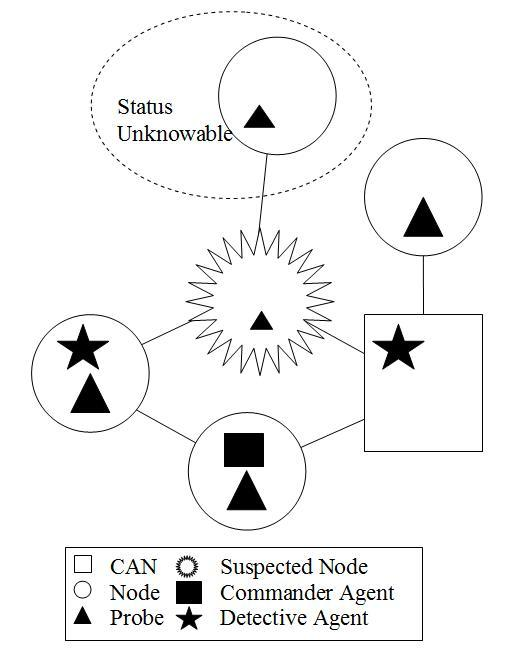
\includegraphics[scale=0.45]{maids}
\caption{The MAIDS Framework}
\label{fig:framework}
\end{figure}

\subsection{Threat Level Two: Network Suspected\\Compromise Investigation}
At this threat level the network is suspected to be compromised.  This triggers the CAN to generate two agent types: a {\it Commander} agent and a {\it Detective} agent.  {\it Commanders} are akin to a localized CAN, the purpose of which is to reduce report latency.  {\it Detectives} are proactive versions of {\it Probes} that communicate observations directly to their {\it Commander}.  The objective is to blockade the suspected node(s) and investigate incoming and outgoing traffic to determine if anomalies are still occurring at a level greater than the threshold value.  Inherently, there is a network effect whereby any node that can only communicate through a suspected node is, of course, also suspect and cannot be trusted (see Figure~\ref{fig:framework}).  Thus, the virtual blockade could indeed comprise a major section of the network.  The CAN takes into account this network effect when placing {\it Detectives} so as not to compromise the aggregate data.  Another important point is that this is merely an investigative roadblock; communication is investigated and monitored but is not stopped.  Again, anomalies are domain dependent, but it makes logical sense that there would be more types of anomalies defined at this level.  Additionally, $T_2$ is the second threshold value of anomaly detection prior to elevation to Threat Level Three.

\subsection{Threat Level Three: Network Compromise Confirmation}
This threat level sees the creation of an additional type of agent, the {\it Secret Agent}, that is essentially something of a sacrificial agent.  Its actions (and the expected results thereof) are predefined; therefore, it can be sent to a compromised node, and if the results are not observed exterior to the node or the communication of its observed effects do not match the observations of {\it Detectives}, then an inference can be made that a compromise has occurred.  It is possible that the {\it Secret Agent} will never be heard from again, in which case this process must be repeated until either the agent survives or a set number of agents have been sacrificed.  It is also possible at this threat level to either elevate to Threat Level Four, or to deescalate if the {\it Secret Agent} is not interfered with.

\subsection{Threat Level Four: Network Compromise Resolution}
For the most elevated threat level, the assumption is that a compromise has occurred.  At this point, there are a variety of actions that can be taken.  The appropriate action is very domain dependent; for example, if resource availability is more important than information security then simply alerting a human while continuing to gather information is the appropriate response.  Alternatively, if information security is more important than availability or redundant resources exist, then automated responses are possible.  The least severe response would be rerouting requests from the compromised node to a sandbox for future analysis and to prevent the compromise of the rest of the network (presumably without making it obvious to the attacker that he has been detected).  A more severe action would be to blockade the node from the network, thereby preventing any requests from leaving or going to that node.  The most severe would be attempting to remove the node from the network or possibly crash it (for example via a distributed denial of service attack or some out-of-band signal).

\section{Pollination}
The proposed pollination scheme in this work is a passive system that allows minimum overhead with active monitoring to provide near real-time discovery of the mobile agent network status.  Pollination involves the exchange of {\it pollen} between the mobile agent and the agency on a node to provide a tracking and a pattern mechanism for use with inference modeling.  The pollen allows the tracking of an individual agent's movements and intentions, and the pollination patterns in both the agent and the node allow for network and agency status to be inferred.  The inference model then classifies the intent, and the security protocols in MAIDS will be enacted based on the perceived intent.  Scaling of the pollination model allows for overhead to be minimized to the level of the threat.

The concept of pollination is designed to create a series of trail markers on both the nodes visited by a mobile agent and the mobile agent itself.  The trail markers allow immediate identification of what nodes the agent has visited by simple inspection of the pollen the agent is carrying.  The inspection of an agent's path via the pollen is performed at its destination.  By traversing the trail of pollen back to the source node one can trace the agent's migration history.

The information provided by pollination is meant to be both historical and active.  Historical information can be used to determine the sequence of events after an event has occurred.  Active information is obtained from real-time inspection and is used to determine if an event has occurred.  For example, in many cases the data and the code that processes it are not singly sensitive.  However, the ability to simultaneously obtain both the data and the code has the potential to cause harm to the agent's designer.  If both nodes are marked, and each node in the network is sensitive to this situation, a mobile agent containing pollen associated with both nodes can be apprehended.

Security in information systems is an important aspect for all applications.  Such security covers three main components: data security, machine security and network security.  One of the key issues involves the authentication of an entity in relation to its access to various resources.  A trusted entity may become compromised, and thus untrustworthy, despite being positively identified.  Determining if an entity has been compromised is an important but complicated process.  The pollination concept introduced in this work extends the capability of MAIDS to detect compromised platforms that passively intercept information.

\subsection{Mobile Agents Pollination}
Mobile Agents Pollination (MAP) is a concept that addresses some of the issues with the MAIDS framework, namely that of detecting passive attacks, by identifying a mobile agent's movements and actions within the network.  MAP uses {\it pollen} to uniquely identify the agencies or groups of agencies on nodes within a network.  Furthermore, MAP uses pollination to form a trail map defining the path an agent utilizes when visiting nodes in the network.  In addition to the trail map, the pollen and map properties can be utilized as action indicators to infer the meaning of the agent's visitations and the intent of agencies within the network.

MAP is similar to the natural process of flower pollination by bees.  Bees traverse a field of flowers to acquire nectar.  When bees encounter a flower, they inadvertently collect pollen from it and distribute pollen to it.  Fundamentally, a grain of pollen represents a flower and a collection of pollen on the bee represents all the flowers it has visited.  The pollen collection left by the bee at each flower represents the sequence of flowers it has visited before encountering the current flower.  The analogy relates to MAP in that the mobile agent is the bee, the nectar is the information (or data) being collected by the agent and the pollen is a node's identification marker.  The role of the mobile agent is to traverse the network of connected nodes to acquire information.  MAP defines the process where the mobile agent {\it unknowingly} collects pollen from the current node and distributes pollen from the previously visited nodes.  The pollen can then be used to quickly infer where the mobile agent has traveled and the sequence of travel.  Other traits related to the map, the pollen, and the pollen's relationship to the nodes can be utilized to expand the perceptibility of the mobile agent's activity in the network.

The main purpose of MAP is to utilize pollination for tracking a mobile agent's activity in the network.  We can then use this tracking information to infer the intent of the mobile agent and the nodes involved in the network.  Ultimately, pollen is a marker used to identify a specific node a mobile agent may visit; pollination is the process of exchanging pollen to provide a mechanism to reconstruct where the agent has been and infer the actions the agent performed.

Pollen can be unique to each node or the pollen can be unique for a subset of nodes depending on user requirements.  The pollen variation throughout the network is similar to the DNA of a flower.  The DNA for a specific node type is mostly the same between entities with minor variations making the sequence unique.  The pollen from two different node types will have a greater variation in the predominating factors.  The pollen strictly provides the identification of a node and should be dependent on the agency configuration to make the process of spoofing it difficult.  The information provided by pollination is meant for both historical and active analysis.  Historical information can be used to determine the sequence of events after an event has occurred.  Active information is used to form real-time inspection in order to determine if an event has occurred.

There are two key observable parameter categories involved in the process of a mobile agent collecting information while traversing the network and visiting nodes: spatial and temporal.  Within MAP, a spatial dimension refers to the network space in the path taken by the mobile agent, the endpoint used by the node, the connection, and the pollen.  Furthermore, this can include the distance of the agent's travel and inter-node distance.  Both are employed by MAIDS.

The network's spatial reference is depicted using standard network nodal reference with connections showing the relation between the nodes.  The pollen associated with the nodes and the agents is represented by unique patterns.  The pollen grains carried by the mobile agent and distributed to the nodes maintain the pattern of the origin node.  The sequence of pollen grains creates a series of trail markers which define the spatial movements of the agent through the network.  A direction depicted by the arrow is inherent in the sequence as the agent migrates from one node to another.  The pattern allows immediate identification of what node(s) the agent visited by simple inspection of the pollen the agent is carrying.  Traversing the trail of pollen defined by the sequence will lead back to the source node.

Within MAP, the temporal dimension is used to refer to the amount of processing a mobile agent expends at a node.  Just as a bee accumulates more pollen the longer it sits at a flower, agents accumulate more pollen the longer they remain at a node gathering data or performing computations.  This may be considered a density in the pollen an agent carries (more {\it grains} of pollen).  The pollen density is associated with the pollen unique to a specific node, and the combination of all the pollen densities will indicate the time taken for the sequence to complete.  A common time reference will maintain a standard gauge for use with the analytics within the MAIDS framework.  The actual time interval is up to the implementation; however, the granularity of the interval should represent the difference between operation actions of the mobile agents for the operations we want to identify.  The temporal reference is depicted by a count below the grains.

We acquire a time-sequence pattern by applying both the spatial and temporal components.  The time-sequence pattern maps the network to the goal of the mobile agent's movement.  The spatial, temporal and spatial-temporal observations are used to infer the meaning of the action with regard to the intent of the agent and nodes.  Associating the content description of the nodes with the pattern may allow for further identification of a mobile agent's actions.

The process of pollination leaves two distinct time-sequence trails as the mobile agent moves from node to node.  The first trail is the set of pollen attached to the agent from the simple process of visiting nodes.  The second is the set of pollen distributed along the path of nodes traveled where each node has a snapshot of the previous nodes the agent has visited.  The sets have a number of key attributes that include node references, number of pollen grains, sequence of grains and the order (or pattern) of nodes visited, and amount of pollen attached.  The pollination concept is depicted in Figure~\ref{fig:map-overview}.

\begin{figure}
\centering
\includegraphics[scale=0.45]{AgentPollen-Example}
\caption{Pollination and Mobile Agents}
\label{fig:map-overview}
\end{figure}

In this figure, an agent is migrating from Node~1 to Node~5.  At each node, the agent exchanges pollen in the process of ``doing work.''  The amount of work is quantified with the temporal reference.  The agent reaches Node~5, and the resulting pattern is depicted with the temporal references denoted by the vector $\left<2, 5, 10, 3\right>$.  Note that Node~6 is not in the agent's path and therefore no pollen is exchanged with this node or the agent.  This example serves as a base pattern or a composite of patterns that can be used to determine anomalies that occur with the agent's or node's standard operation.

\subsection{Usage of Mobile Agents Pollination in\\MAIDS}
In order to address passive attacks we simply need to have analytics to infer the meaning of the change in pattern.  For example, suppose that a passive node successfully inserts itself into the network.  The node will have to understand that pollination occurs otherwise it will not be accepted.  We assume the attacker is smart enough to spoof a node (and understand that pollination occurs but not necessarily how it works) and continue with more advanced security concerns.

\begin{figure}
\centering
\includegraphics[scale=0.45]{AgentPollen-PassivenodeA}
\caption{Network with Passive Node}
\label{fig:map-eg}
\end{figure}

Suppose we mark the path agents would take from Node~1 to Node~4 (see Figure~\ref{fig:map-eg}) by marking each of the intermediate nodes with different pollen.  Every time an agent reaches Node~4, it possesses a sequence of pollen that corresponds to the path taken.  This is verified with the sequence that the agent was supposed to follow in order to determine if the agent has been compromised by an additional passive node or a violation of the agent code.  The passive node is identified by added pollen, incorrect pollen or simply the lack of pollen in the sequence inspected at the destination node.  A team of {\it Commanders} and {\it Detectives} can be used determine which node is the passive node and eliminate it.  Compromised agents can simply be eliminated from the system at Node~3 upon arrival and trigger the inspection.  For added security, every node along the path checks the pollen sequence and essentially provides a passive defense mechanism against corruption.

\subsection{Implementation}
The pollination process works at the application level where the agencies represent the nodes and mobile agents move throughout the network migrating from node to node.  The nodes each have their own unique pollen definition.  Implementing the pollen requires the ability to attach pollen and transport it with the mobile agent; it is {\it picked up} and {\it dropped off} by the nodes.  We propose that the process of attaching the pollen to the mobile agent is not performed by the agent itself in order to maintain a correlation to the natural process of pollination (with bees and flowers).  The agent should not know or care about how pollination works.  We envision the use of a manipulation of the Open System Interconnection (OSI) \cite{wetteroth01} model's transport layer for both attaching the pollen to the agent and transporting the pollen and agent to the destination node.  In the OSI model, the application data to be transported is broken into packets and transmitted from source to destination.  We can add additional packets by appending the pollen to the data stream, or we can manipulate the packets using packet tagging (e.g., \cite{belenky03, djemaiel07}).  Adding additional packets can be accomplished at the application level by simply appending to the end of the mobile agent in that data stream.  The addendum is removed at the node and the pollen is recovered.

Packet tagging is accomplished by marking packets with identifiers for local purposes.  The actual mark is part of the packet and cannot be removed; however, the mark can be modified or replaced with another mark.  This may be an issue if the agent is transmitted to some location that is external to the system (outside the view of the MAIDS framework).  However, for our purposes the mobile agent is assumed to remain internally within the network.

In addition to the pollen tag itself, the count representing action at each node can be used to acquire further insight into the meaning of the agent's intent.  It is expected that a node with little information to share will require less time for the mobile agent to visit the node (i.e., less activity).  Using the activity gauge, we can infer some of the intent of both the agent and the node.  In the example of a passive node scenario, we can expect the sharing to be minimal for the agent (as described by the label ``0'' in Figure~\ref{fig:map-eg}) with regard to the passive node's pollen.

The reverse is also possible with the relationship between the node's pollen and the data stored at the node.  Using this relationship between the information of the node with the highest activity, we can infer the type of information the agent is interested in gathering and the information with little interest.  The entire concept is depicted in Figure~\ref{fig:map-eg}.  The purpose of pollination is to allow an easy identification method for activity within a multi-agent system using pollination patterns.  Any standard inference model (e.g., fuzzy logic, neural network, Bayesian model) can be utilized to trigger MAIDS security events from the pollination patterns.

A variation of the scheme can be implemented to acquire different levels of security throughout the network.  At a low level we are only concerned with sensitive data or applications.  For this we simply need to pollinate those locations and track the movement of agents carrying that pollen.  Nodes are always active to interpret the meaning of the mobile agents and the surrounding nodes.  The limitation of the pollination to a subset of the network has the effect of greater focus-ability on only the things that matter.  This, in turn, has the effect of reducing the overhead associated with pollination in both time and space.  Furthermore, we can change the pollination patterns associated with the network on a periodic basis to ensure security.  This change can either be notified to the MAIDS security team in advance or it could simply trigger an event that allows the team to determine the appropriate action.  The latter is preferable as the addition of a mechanism to disable security for changing patterns could be an exploitable vulnerability.  The event triggered by the pattern change can be used as a test of system integrity as the process goes through the threat levels and back to Threat Level One.

The state of the system primarily resides at Threat Level One; however, as security concerns increase, the number of pollinated nodes increases to match the threat.  The increase can either be tactically focused on the relative sensitivity of the data or it can be distributed throughout the network to provide a ``big picture'' of the secured environment.  At the highest level all nodes will be pollinated, and nodes without pollen or agents not containing pollen will be apprehended.  The pollination paths not adhering to the required patterns will be examined to determine what events took place by the MAIDS security team.

\section{Detecting Passive Nodes with\\Pollination}
Pollination is a tool that provides input into the MAIDS framework.  Fundamentally, this input provides an additional data set that can be used for anomaly detection.  For instance, pollen appearing from ``new'' nodes that should not exist may indicate an intruder connected to the network wirelessly.  Alternatively, a drastic and sudden change in traceroutes for the network may indicate abuse.  These anomalies feed naturally into the existing MAIDS threat levels.

In addition to pollen serving as a data source, traps can periodically be set in order to lure passive nodes to actively search for phantom prized data that, in turn, will expose their cover.  As part of this process, the CAN will elevate the threat to Threat Level Two and randomly select a set of strategic nodes of interest (SNI) throughout the network as the host of the prized phantom data.  Each trap will have a designated area of effect that determines the number of nodes that are affected.  The CAN will then send agents to each node with the objective of broadcasting the existence of crucial data in the SNI.  When a request for the phantom data is received at the SNI, the network threat will be elevated to Threat Level Four and the CAN will backtrack the pollen pattern to the originating host, marking it as a suspected compromised host.

\subsection{The ``Mole'' Scenario}
We have illustrated the use of pollination within MAIDS to assist in the detection of passive nodes (and attackers).  However, there are many other uses for pollination; such a method can be used to detect other kinds of attacks.  Take, for example, an insider threat and consider the following scenario: an organization's management is noticing that its main competitor frequently releases a product that is very similar to and directly competing with releases of their own--and it is doing so a few weeks prior to its own release dates.  One might suspect that an insider is leaking information (and possibly being paid for it).  How might the management of this organization determine if this is indeed happening and, if so, who is leaking the intellectual property?

By implementing MAIDS with pollination within the organization's network, we would be able to detect such an event and narrow down the leak to a subset of nodes (and possibly determine who the leak is).  The solution requires an approach from two directions: from within the MAIDS framework and from a social engineering standpoint.  One technique to identify an insider threat might be to announce the forthcoming release of a fictitious product whose details are located on a server (or servers) that resides at a particular node (or a subset of nodes) in the network.  As previously stated, the CAN will randomly select a set of SNIs throughout the network that will host the fictitious information.  Clearly, the fact that the product is fictitious and will never actually be released is something the management will conceal; this is the social engineering component of the approach.  The idea is to entice the leak to obtain the details of the product while using the MAIDS framework with pollination to identify him.

Pollen is something that uniquely identifies nodes; so to determine the agents that are accessing the fictitious information, we simply generate a unique pattern on the SNIs that provide this information.  There is no need to pollinate from other nodes in the network, as we are uninterested in them at the moment.  Now we simply need to track those agents that are carrying the pollen.  Once pollen is being carried around by the agents and is stored on the nodes in the network, we can inplement a set of traps that will assist in detecting the leak.  Since nodes are always active to interpret the meaning of the agents and the surrounding nodes, MAIDS can focus on the leak.  Agents sent by the CAN roam through the network in search for the pollen.  When they find it, the CAN will raise the network situational awareness to Threat Level Two and proceed to investigate the path taken by the agent to reach the SNI.  Instead of attempting to determine compromised nodes, {\it Commanders} and {\it Detectives} will be looking to locate the source of the information request in order to extirpate the source node--and thus the insider threat.

\subsection{The Packet Sniffer Scenario}
Consider the case when an attacker simply wishes to passively sniff for interesting packets in the network.  In order to do so, the attacker must successfully (and secretly) insert a node in the network.  In the case that the attacker has no idea that pollination is being utilized, he will be easily detected.  As agents go through the attacker's node, they will go through un-pollinated, and this will be detected at some other node in the agent's path.  This is illustrated in Figure~\ref{fig:map-eg}.

But suppose that the attacker has some knowledge that a pollination scheme is being implemented in the network.  The pollen being generated at his node will be unrecognized in the agent's pollination sequence (i.e., it is not pollen that the framework knows anything about).  And again, the attacker will be easily detected.

In the most unlikely case, an attacker may clone the pollen being generated at some other (legitimate) node in the network.  Since pollen for a node is randomly generated (and may change frequently), it is very unlikely that this will happen; however, this occurrence can still be detected by MAIDS as the pollen sequence will contain the same pattern more than once in the vector (and out of order).

\section{Conclusion and Future Work}
The MAIDS framework previously introduced (in \cite{kackley09}) provides the ability to detect, investigate and deal with compromised nodes utilizing a multi-agent scheme in an effective and efficient network intrusion mechanism.  However, MAIDS relies heavily on nodes that actively attempt to obtain data that they are not entitled to (and tipping their hand in the process).  In the event that an intruder remains passive and only collects data that it unwittingly comes across, MAIDS is unable to detect it.  To address the detection of passive attackers, incorporating pollination into the MAIDS framework was proposed.  As an added bonus, pollination also provides additional forensic capabilities in that a reconstruction of what occurred (i.e., where an agent migrated throughout the network) is possible.

As this work is still very new, there are a large number of areas we may explore in order to further improve MAIDS.  The role of pollen can be expanded and could, for example, affect an agent's functionality or modify the data it collects thereby rendering it useless.  When a node encounters pollen it does not recognize, it can either refuse the agent, respond to the agent's request (should it make one) with misinformation, or cease future communication with the node that supplied the pollen.  Alternatively, we could embed information in the pollen via a predetermined set of pollen ``colors'' or patterns.  These could represent different hidden emergency messages that can be relayed by each host to the CAN.  This simple coloring scheme can act as a silent alarm that notifies the CAN for a possible breach in one or more nodes.

In reference to the purposeful setting of traps in order to lure potential passive attackers, we noted that when such a trap is sprung, the threat level elevates from Threat Level Two directly to Threat Level Four.  This is somewhat drastic, but it is difficult to imagine a way of further confirming that a passive attacker exists without human intervention.  Additionally, the amassed evidence will be fairly incriminating.  It may eventually be possible to engineer a {\it Secret Agent}, as in Threat Level Three, capable of further investigation in an attempt to confirm this.  It is unclear what exact form this would take, but it merits investigation.

As noted, the purpose of pollination is to allow an easy identification method for activity within a multi-agent system using pollination patterns.  Any standard inference model (e.g., fuzzy logic, neural network, Bayesian model) can be utilized to trigger MAIDS security events from the pollination patterns.  Such a discussion of models (and perhaps the {\it best} model) is not provided in this paper but merits attention in the future.

\nocite{*}
\bibliographystyle{abbrv}
\bibliography{sigproc-sp}  % sigproc.bib is the name of the Bibliography in this case

\balancecolumns
% That's all folks!
\end{document}
